\section{Recurrent Neural Networks}\label{RnnLstm}
If we feed a network with a string, it produces a binary vector as an output.
Consequently, the order of the words are lost.
Recurrent Neural networks are kind of language encoder, that can process the sequence of data.
The recurrent layer of an \ac{RNN} re-introduces the words order into the networks internal.
Furthermore, the inputs are distinguished chronologically by an index $t: x_{t-1},x_t, x_{t+1}$.
And a second matrix $U$, such that values can be sent to the next layer is used \cite{haralambous_course_2024}:
\begin{equation}
    \sigma(Ax_t+Ux_{t-1}+b)
\end{equation}

The architecture of \ac{RNN}, is illustrated in Figure \ref{fig:RNN}.
It implies that the temporal sequence of the input data has an influence on the result.
For this purpose, information from one processing step is transferred with a time delay to the processing of the next one using the following pattern.

\begin{figure}[h]
   \centering
   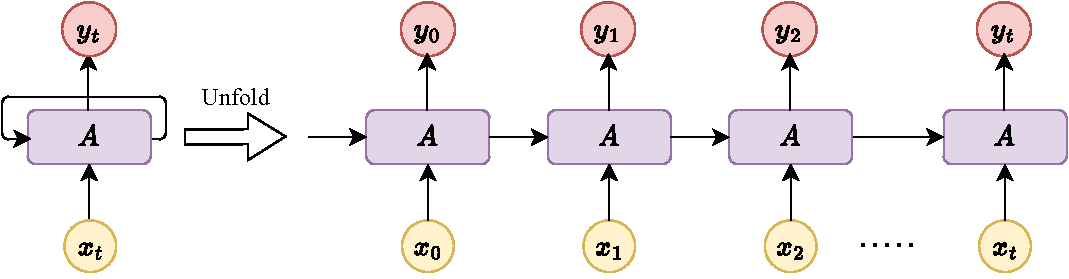
\includegraphics[width=0.8\linewidth]{Abschlussarbeit/Pictures/RNN.drawio.pdf}
   \caption{\ac{RNN}, output of first influences the second \cite{BiLSTM}}
   \label{fig:RNN}
\end{figure}

Especially with backprobagation, \ac{RNN}s have the disadvantage that the gradients either vanishes or explode if the length of the sequence is long enough.
This leads to a very slow manner of the models training.
When this occurs, \ac{LSTM} networks can help. 
They are a type of \ac{RNN} architecture that uses an internal memory that stores the inputs that were fed to the model at previous time steps.

Ideally, this will solve the problem of the disappearing or exploding gradient.

\ac{RNN} can only process word by word and this is why they are operating very slow, compared to transformer, that are able to process a complete sentence 
\ac{LSTM} \cite{originalLSTM_book} are special \ac{RNN} cells, that uses an internal memory and multiplicative gates.
As Smagulova and James \cite{LSTM}, we explain \ac{LSTM} by the use of figure \ref{fig:LSTM}, that illustrates the unit architecture of an original \ac{LSTM} with memory cell and two gates. 

\begin{figure}[htb]
\begin{minipage}{7.5cm}
 \centering
   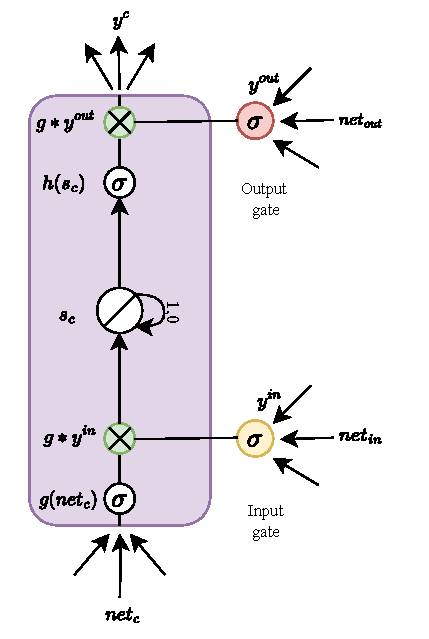
\includegraphics[width=\linewidth]{Abschlussarbeit/Pictures/LSTMoriginal.pdf}
   \caption{Original \ac{LSTM} \cite{LSTM}}
   \label{fig:LSTM}
\end{minipage}
\hfill
\begin{minipage}{6.5cm}

The self-connected linear unit, denoted by $s_c$, which is also called constant error carousel, the hear of a memory block.
The input gate, with weighted inputs, is denoted as $net_{in}$ and the output as $y^{in}$
The output gate with weighted input is denoted as $net_{out}$ and $y^{out}$ shapes the output of the cell $y^c$.
$h$ is a differentiable function, that scales $x_c$.
$g$ is a function, that squashes the weighted input of the cell $net_{c}(t)$.
\end{minipage}
\end{figure}


Originally, \ac{LSTM} is subjected to some limitations due to the linear nature of $s_c$.
Consequently, a forget gate layer was included to delete and forget unneeded information. 
There is a similarity between the behaviour of \ac{LSTM} cell with forget gate and the standard \ac{LSTM} with exception of cell state/ internal memory $s_c(t)$/ $c_t$, which includes an impact of an output of the forget gate $y^\varphi/f_t$.
We can define the two parameters as follows:

\begin{equation}
    \begin{split}
            & s_{c_j}(t) = y^{\varphi_j} (t) s_{c_j(t-1)}+y^{in_j}(t)g(net_{c_j}(t))\\
            \\
            & y^{\varphi_j}(t)=f_{\varphi_j}(net_{\varphi_j}) 
    \end{split}
\end{equation}


The forget gate's behaviour is similar to standard \ac{LSTM}.
In this process, the cell input $x_t$ at time $t$ concatenates with output $h_{t-1}$ of the previous cell at previous time step $t-1$.
$h_{t-1}$ is denoted by hidden state. 
The resulting vector traverses input nodes $g_t$, forget gate $f_t$, input gate $i_t$ and output gates $o_t$.
Afterwards, the forget gate decides whether the cell data $c_{t-1}$ from a previous time step will be kept or blocked.